\graphicspath{ {./1-supervised-learning/} }

\chapter{Supervised Learning}


As stated earlier, in the supervised learning framework, the goal is to train a model to learn a relationship between datapoints and their corresponding labels from a sample of datapoints drawn i.i.d. from some fixed distribution $\mathcal{D}$. To evaluate the accuracy of our model, we define a loss function which evaluates how dissimilar a model's prediction is on a datapoint from the truth.


In supervised learning, training data is used to train a model, and a trained model can make predictions on observations. The goal is to learn predictions that are close to the true (often unobserved) $y$.

\begin{figure}
\centering
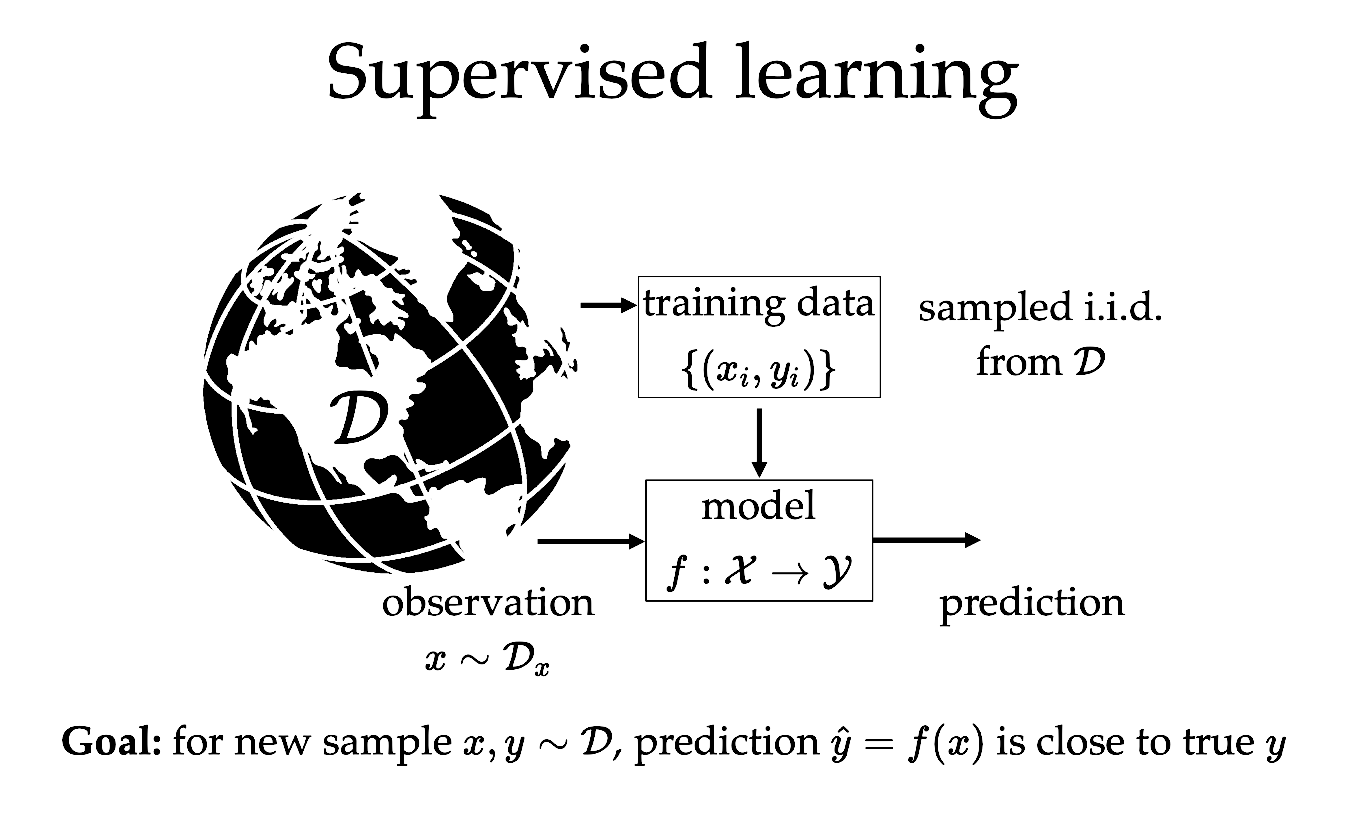
\includegraphics[width=3in]{graphics/sup_learning.png}
\caption{Supervised Learning, from the Lecture 1 slides.}
\end{figure}

The goal of supervised learning can be formalized as a risk minimization problem.
Given some user defined loss function $\ell$, the goal in risk minimization is 

\begin{equation}
\min_{f \in \mathcal{F}} \mathcal{R}(f) = \mathbb{E}_{x, y \sim \mathcal{D}} [\ell(y, f(x))]
\end{equation}

where $\mathcal{D}$ is a dataset and $\mathcal{F}$ is the set of candidate models. When we approximate $\mathbb{E}_{\mathcal{D}}$ with an actual dataset and evaluate $R$ over real data points then this becomes empirical risk minimization.
The process of supervised machine learning can thus be encapsulated in two things: defining a loss, and conducting risk minimization. 

\section{Loss Functions}
A loss function $\ell(y, \hat{y})$ measures the loss when a model predicts $\hat{y}$ when the true label is $y$; this function varies on the setting and desired characteristics of the learning algorithm.  

\begin{table}[ht] 
\centering
  \fontfamily{ppl}\selectfont
  \begin{tabular}{p{0.3\linewidth} | p{0.7\linewidth}}
    \toprule
    Classification Loss & Usage \\
    \midrule
    \textbf{Zero-One Loss} $\mathbb{1}[y\not=\hat{y}]$ & Classification accuracy; this loss is non-continuous and impractical to optimize because of its non convexity. \\
    \textbf{Hinge Loss} $max(0, \hat{y} - y)$ & Denotes the margin between the linear separator and its closest points on either class, it is convex but isn't differentiable at $\hat{y}=y$.  This is used in the standard SVM. \\
    \textbf{Log Loss} $log(1 + e^{-\hat{y}y})$ & Outputs are well-calibrated probabilities for each class; this loss function is used for logistic regression. \\
    \textbf{Exponential Loss} $e^{-\hat{y}y}$ & Used in AdaBoost, misprediction loss increases exponentially: this can converge quickly or cause issues when the data is noisy. \\
    \bottomrule
  \end{tabular}
  \caption{Different classification losses can be picked to handle different optimization schema.}
  \label{tab:normaltab}
  %\zsavepos{pos:normaltab}
\end{table}

\begin{table}[ht] % if you can make the equation and name work well on the same line, idk how to do that tho it isn't that important
  \centering
  \fontfamily{ppl}\selectfont
  \begin{tabular}{p{0.3\linewidth} | p{0.7\linewidth}}
    \toprule
    Classification Loss & Usage \\
    \midrule
    \textbf{Mean Absolute Error} $\left|f\left(\mathbf{x}_{i}\right)-y_{i}\right|$ & Estimates median label: this loss function is convex and less sensitive to noise but it isn't differentiable at 0. \\
    \textbf{Squared Loss} $\begin{aligned}
&\left(f\left(\mathbf{x}_{i}\right)-y_{i}\right)^{2} 
\end{aligned}$ & Estimates mean label: this loss function is convex and differentiable everywhere, but it's sensitive to outliers and noise. \\
    \bottomrule
  \end{tabular}
  \caption{Different regression losses can also be picked to handle different optimization schema.}
  \label{tab:othertab}
  %\zsavepos{pos:normaltab}
\end{table}

% \includegraphics[width=\linewidth]{graphics/Loss_reg.png}

%   - regression: |^y-y| MAE, (^y-y)^2 MSE both convex, square is also smooth 

\section{Risk}

\marginnote{Risk can be seen as a natural lens to view a model's predictive power.} 

As loss is a function that is highly dependent on the sample it has received, we define a new concept to better capture the robustness of a Machine Learning model. The risk of a predictor $f$ over a distribution $\mathcal{D}$ is the expected (average) loss. Risk is mathematically defined in the following way:

$$\mathcal{R}(f)=\mathbb{E}_{x, y \sim \mathcal{D}}[\ell(y, f(x))].$$
\newline 

\noindent

\begin{claim}
    The predictor with the lowest possible risk is: \sidenote{If we have the true distribution of labels (an entry for everyone in a population), setting a threshold/cutoff will give us the best classifier! Unfortunately, this usually isn't realistic as in the real world.}
    \begin{itemize}
        \item $\mathbb{E}[Y \mid X]$ for squared loss
        \item $1\{\mathbb{E}[Y \mid X] \geq t\}$ for $0-1$ loss, with threshold $t$ depending on $\mathcal{D}$
    \end{itemize}
\end{claim}


\begin{proof}

\noindent
  This can be proven using the tower property of expectation, also known as the law of total expectation. 

\begin{fact}
The Law of Total Expectation states that if $X$ is a random variable whose expected value $\mathbb{E}[X]$ is defined, and $Y$ is any random variable on the same probability space, then $\mathbb{E}[X] = \mathbb{E}[\mathbb{E}[X|Y]]$.
\end{fact}

\noindent
Giving loss $\ell(f(X), Y)$ of a model on a dataset as a random variable with $X$ as another random variable in the same probability space, we can use this fact to expand:

$$
\mathbb{E}_{X, Y \sim \mathcal{D}}[\ell(f(X), Y)]=\mathbb{E}_X[\mathbb{E}_Y[\ell(f(X), Y) \mid X]]
$$


\newthought{For a squared loss} we can plug in $\ell(f(X), Y) = (f(X) - Y)^2$, and we may thus say that we are looking for 
$$\hat{f} = \argmin_f \mathbb{E}_X[\mathbb{E}_Y[(f(X) - Y)^2 \mid X]]$$

\noindent
Since squared loss is convex and the minima of a convex function can be found at the point where the derivative is zero, we may find that:
\begin{align*}
    \frac{d}{df(X)} \mathbb{E}_X[\mathbb{E}_Y[(f(X) - Y)^2 \mid X]] &= 0 \\
    \mathbb{E}_X[\mathbb{E}_Y[2 (\hat{f}(X) - Y) \mid X]] &= 0
\end{align*}

\noindent
By linearity of expectation, this gives us $\hat{f}(X) = \mathbb{E}_Y[Y | X]$
\begin{align*}
    \mathbb{E}_X [\mathbb{E}_Y[2 (\hat{f}(X) - Y) \mid X]] &= 2 (\mathbb{E}_X [\mathbb{E}_Y[\hat{f}(X) \mid X]] - \mathbb{E}_X [\mathbb{E}_Y[Y \mid X]]) \\
    &= 0 \\
    \mathbb{E}_X [\mathbb{E}_Y[\hat{f}(X) \mid X]] &= \mathbb{E}_X [\mathbb{E}_Y[Y \mid X]] \\
    \hat{f}(X) &= \mathbb{E}_X [\mathbb{E}_Y[Y \mid X]]
\end{align*}

% If we only look at the inner expectation and consider our X random variable set to a random value x, we can rewrite our f(X) as f(x) - not a random variable anymore - the variability that we are interested in here is only due to our choice of function in our minimization problem. Let's now just rename this f(x) as a variable z which varies with the function f that we will choose in our minimization problem. Our minimization problem is therefore the following:\\
% $$\hat{z} = \argmin_{z\sim Z} \mathbb{E}_Y[(Z - Y)^2 ]$$

% \noindent
% If we take the derivative over z and find $\hat{z}$ we end up solving:
% $$\mathbb{E}_Y[2(\hat{z} - Y) ] = 0$$
% By linearity of expectation, we get:
% $$\hat{z} = \mathbb{E}[Y]$$
% Coming back to our initial problem, we were looking for the optimal predictor $\hat{f}(x)$.
% Reinjecting x as a variable, our problem ends up being:
% $$\hat{f}(x) = \mathbb{E}[Y \mid X]$$


\newthought{For a 0/1 loss} we can take advantage of the fact that $f(x) \in \{0, 1\}$ to expand the inner expectation:


$$\begin{aligned}
&\mathbb{E}_Y[\ell(0, Y) \mid X=x]=\ell(0,0) \mathbb{P}[Y=0 \mid X=x]+\ell(0,1) \mathbb{P}[Y=1 \mid X=x] \\
&\mathbb{E}_Y[\ell(1, Y) \mid X=x]=\ell(1,0) \mathbb{P}[Y=0 \mid X=x]+\ell(1,1) \mathbb{P}[Y=1 \mid X=x]
\end{aligned}
$$

\noindent
Since it is a 0/1 loss, $\ell(1,0) = \ell(1,0) = 1$ and $\ell(0,0) = \ell(1,1) = 0$ so this expansion simplifies to:

$$\begin{aligned}
&\mathbb{E}_Y[\ell(0, Y) \mid X=x]= \mathbb{P}[Y=1 \mid X=x] \\
&\mathbb{E}_Y[\ell(1, Y) \mid X=x]=\mathbb{P}[Y=0 \mid X=x]
\end{aligned}
$$
We are looking for the predictor that will always predict the smaller of these two terms for a given x (since we are trying to minimize this inner expectation for our overall risk). We want to predict $0$ if $\mathbb{P}[Y=1 \mid X=x] \leq \mathbb{P}[Y=0 \mid X=x]$ and $1$ if $\mathbb{P}[Y=1 \mid X=x] \leq \mathbb{P}[Y=0 \mid X=x]$.

\noindent
We can use this to rewrite:
$$\hat{f}(x) = 1\{\mathbb{P}[Y=1 \mid X=x] \geq \mathbb{P}[Y=0 \mid X=x]\}$$

\noindent
From the property that $Y \in \{0, 1\}$, we can use $\mathbb{P}[Y=1 \mid X=x] + \mathbb{P}[Y=0 \mid X=x] = 1$ to simplify this expression:
$$\hat{f}(x) = 1\{\mathbb{P}[Y=1 \mid X=x] \geq 1 - \mathbb{P}[Y=0 \mid X=x]\}$$ 

\noindent
By the definition of expectation, we simultaneously have:
\begin{align*}
\mathbb{E}[Y \mid X = x] &= 1*\mathbb{P}[Y=1 \mid X=x] + 0*\mathbb{P}[Y=0 \mid X=x] \\
&= \mathbb{P}[Y=1 \mid X=x]
\end{align*}
Putting this all together and setting $t = 1 - \mathbb{P}[Y=0 \mid X=x]\}$ we get:
$$\hat{f}(x) = 1\{\mathbb{E}[Y \mid X = x] \geq t \}$$
\end{proof}
% \textbf{Proof:} 


\section{Prediction errors}\label{sec:prediction_errors}
Loss determines trade-offs between errors, as some variation might be truly unexplainable or our feature set might not be complete!  An example of this might be attempting to predict whether a person in a picture is sitting or standing simply based on the position of their face in a frame.  This feature set clearly won't give us a 100\% accurate classifier. 

When we classify, we might classify things correctly (predict stand for a standing person, sit for a sitting person), and here it would make sense for the loss to be 0; however, what if we predict standing for a sitting person versus sitting for a standing person?  Would we want to assign both these situations the same loss?  We must make this decision based on the motivation of building our model, and based on our priorities.  

An example of where we might want to bias this is the proposed idea for skipping TV advertisements in the future: the idea proposed that people could stand up during an ad, and a camera would capture this movement and skip it.  Perhaps we care about customer satisfaction, so we might want to give a higher loss to predicting sitting when the person stands, so customers wouldn't return TVs which force them to stand multiple times to skip an ad.  Perhaps we care more about advertiser satisfaction, so we might want to give a higher loss to predicting standing when the person sits, so we can ensure that consumers won't accidentally skip ads which they might have acted upon while idly sitting.  There are many things to consider for each decision while designing a loss function!

In many domains, decisions have moral and legal significance, and harms can occur at many levels.  As machine learning is applied to a variety of settings, we must analyze several possible ways that machine learning algorithms might cause harm in application.  \\

\begin{itemize}
    \item Correctness: who is burdened by errors?
    \item Stereotyping: which correlations are permissible?
    \item Specification: who is left out?
\end{itemize}

An additional component of these issues is that we don't often have access to the entire population $\mathcal D$ and instead use a finite dataset; we revisit this issue towards the end of the chapter.





\section{Fairness Metrics}

Consider the problem of targeted job ads\footnote{\url{https://www.theverge.com/2018/10/10/17958784/ai-recruiting-tool-bias-amazon-report}}, where we want to tell targeted users that we are hiring a programmer. If we use demographic information and browsing history as our input features $x_i$ and whether or not the user clicked (1) or not (-1) as our label $y_i$, we can use the following linear model to determine whether or not to serve ads to future users.

$$\hat{\theta} = \argmin \sum_{i=1}^{N} (-\theta^Tx_i \cdot y_i)_+ \hspace{1cm} \hat{f}(x) = \mathbb{1} \{\hat{\theta}^Tx \ge t\}$$

However, if we optimize this model, we may find that the index of $\hat{\theta}$ corresponding to ``visited website for women's clothing store'' is negative, which implies some sort of bias in the model. We can try to resolve this by removing the feature for women's clothing, but this will just result in other features being selected that may result in biased models. Clearly, removing features that are potentially problematic is not a solution, and this phenomena is known as ``no fairness through unawareness.'' 

\subsection{Statistical Classification Criteria}
\begin{marginfigure}
\centering
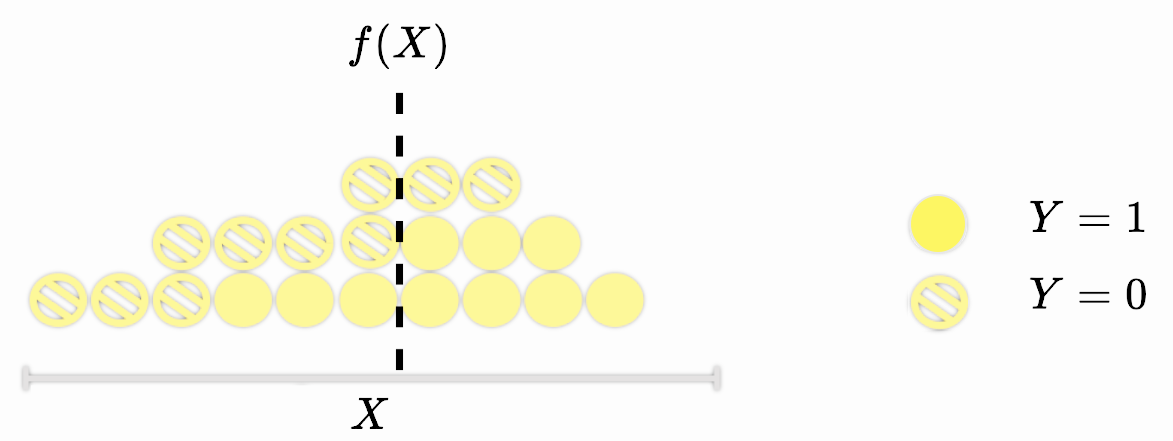
\includegraphics[width=\linewidth]{graphics/example.png}
\caption{Examples of statistical classification criteria.}
\end{marginfigure}
A key component of measuring fairness is understanding what and when the model is predicting. 
Here we demonstrate some metrics that describe this along with an example:
\begin{center}
\begin{tabular}{ ||c | c|| }
 \hline
 Accuracy: $\mathbb{P}(\hat{Y} = Y) = 0.75$  & Positive Rate: $\mathbb{P}(\hat{Y} = 1)= 0.45$ \\ 
 False Positive Rate: $\mathbb{P}(\hat{Y} = 1 | Y = 0)=0.2$ & False Negative Rate: $\mathbb{P}(\hat{Y} = 0 | Y = 1)=0.3$ \\  
 True Positive Rate: $\mathbb{P}(\hat{Y} = 1 | Y = 1)=0.7$ & True Negative Rate: $\mathbb{P}(\hat{Y} = 0 | Y = 0)=0.8$\\
 Positive Predictive Value: $\mathbb{P}(Y = 1 | \hat{Y} = 1)=\frac{7}{9}$ & Negative Predictive Value: $\mathbb{P}(Y = 0 | \hat{Y} = 0)=\frac{8}{11}$\\
 \hline
\end{tabular}
\end{center}

\subsection{Fairness Frameworks}

Here we discuss some frameworks for assessing fairness, a rough idea of the methods to integrate fairness into our model, and the limitations of these methods. Further we mention other instances of discrimination in non classifier models:\\
Due to the biases that risk minimization models develop, we need some additional criteria besides the loss function to achieve fairness. e.g. in the targeted ad example above, the goal is to treat individuals roughly the same across groups. To formalize that, we present 3 criteria that measure this goal:
\begin{itemize}
    \item \textbf{independence:}\\ equalizes positive rate across groups; prediction does not depend on attribute. $\hat{y} \perp a$\\
In the context of the example above, we look at individuals from different racial categories and want to see that predictions look the same, i.e show the ad at equal rate across gender. However, there might be scenarios where this criteria doesn't seem appropriate. As an example, if the predictor is whether somebody is currently pregnant and we would like to show pregnancy-related ad and baby ads. Since there is some underlying difference in pregnancy across genders, this is not the right criteria.
    \item \textbf{separation:}\\ equalizes error rate across groups; given outcome, prediction does not depend on attribute. $\hat{y}\perp a\, \vert y$\\
    in the example, the ad in this case should be displayed to interested users at equal rates across gender. Here by conditioning on the actual outcome, we allow ourselves to account for the fact that certain properties of interest might differ across these protective attributes.\\
    This is relying on what the true qualification level in a population is, or what the underlying distribution of your labels is.
    \item \textbf{sufficiency:}\\ equalizes predictive value across groups; given prediction, outcome does not depend on attribute. $y\perp a\, \vert \hat{y}$\\
    This is saying your predictions are equally useful across all groups by race, or gender or disability, status, or whatever the particular attribute encodes. In the ad example, the users who end up having the ad display to them are interested at equal rates across gender.\\
    This is focused less on the truth of the population, and more on the truth in the model, which is what we're designing. We just want to improve that.
\end{itemize}
\subsection{Achieving non-Discrimination Criteria}
to achieve these fairness criteria we need to process data, the methods are:

\begin{itemize}
    \item \textbf{preprocessing:}\\ The benefit of this is diagnostic to the downstream tasks, and it gets rid of any correlations that could otherwise be used, yet it might end up making accuracy hard to achieve. And it requires knowledge of attributes during data pruning.\\
    in the example illustrated in the picture this corresponds to shifting the data itself.
    \begin{figure}
    \centering
    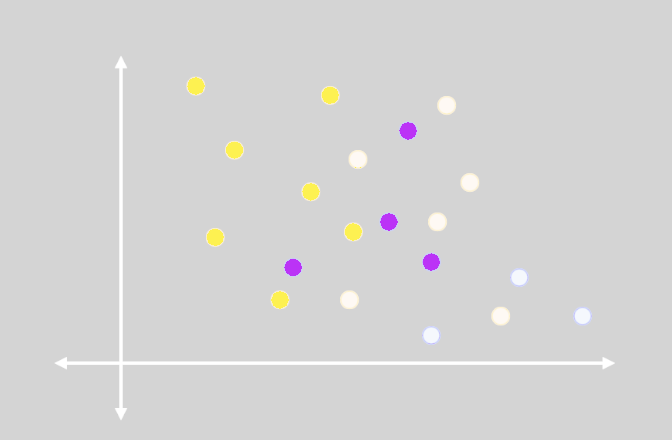
\includegraphics[width=.3\textwidth]{graphics/p1.png}
    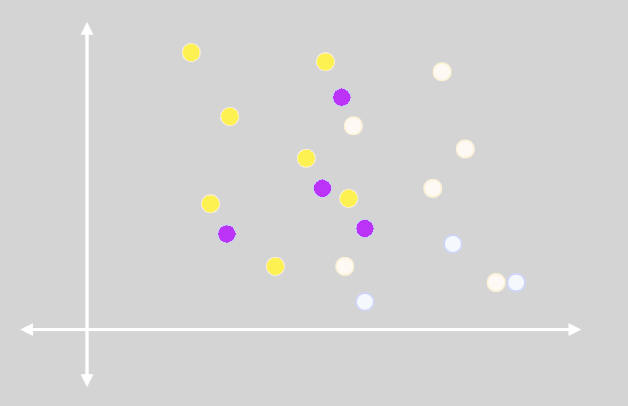
\includegraphics[width=.3\textwidth]{graphics/p2.png}
    \caption{data befor and after pre-processing}
    \end{figure}
    
    \item \textbf{inprocessing:}\\
     Where you change the learning algorithm itself with respect to these criteria, with respect to these criteria, this one will require that you know the protected attribute during training time.\\
     so in the example instead of drawing a linear boundary, we would draw a more complicated looking boundary that will actually satisfy the independence criteria, i.e. equal acceptance rate across groups.
    \begin{figure}
    \centering
    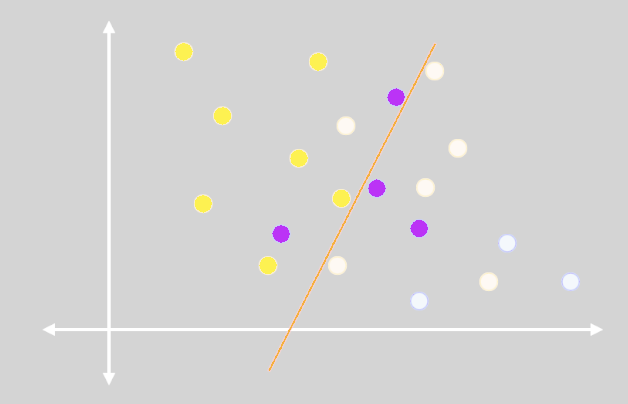
\includegraphics[width=.3\textwidth]{graphics/p4.png}
    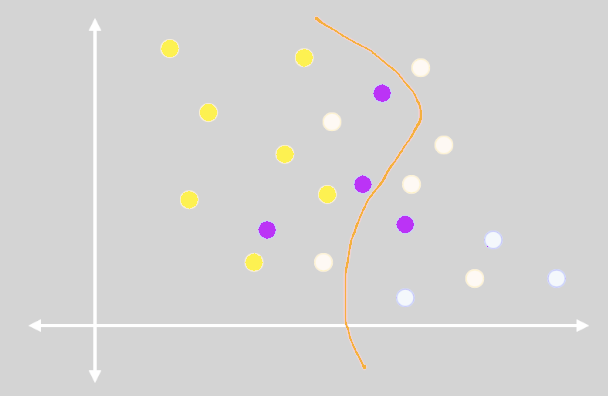
\includegraphics[width=.3\textwidth]{graphics/p3.png}
    \caption{the linear boundary and the boundary after in-processing}
    \end{figure}
    \item \textbf{post processing:}\\ Where we train a model normally and adjust the thresholds(for binary classification) in a group dependent manner after that. This requires incorporating protected attributes at decision time. example.\footnote{See \url{https://research.google.com/bigpicture/attacking-discrimination-in-ml/} for an interactive post processing example.}
    \vspace{10mm}
    \begin{figure}
    \centering
    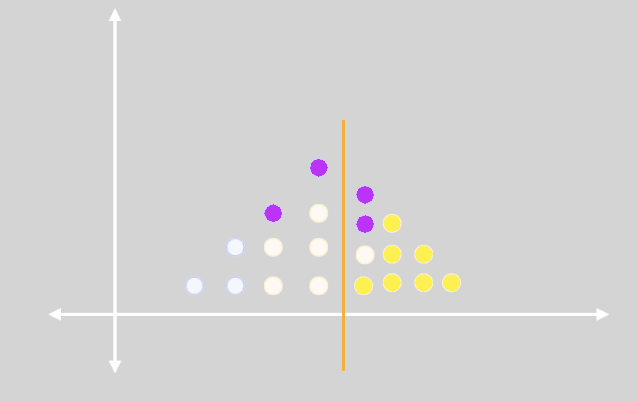
\includegraphics[width=.3\textwidth]{graphics/p5.png}
    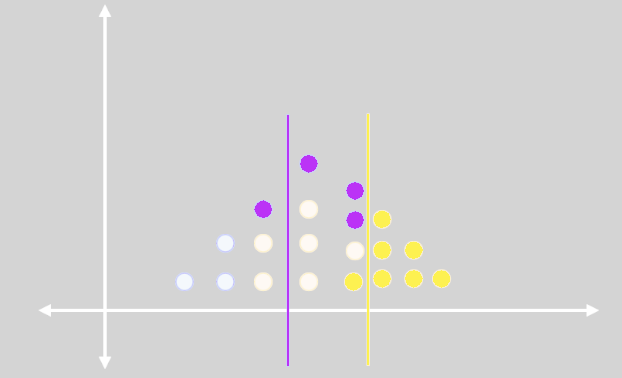
\includegraphics[width=.3\textwidth]{graphics/p6.png}
    \caption{linear classifier without and with post-processing}
    \end{figure}
\end{itemize}
These non-discriminative criteria have some limitations, to mention a few:
\begin{itemize}
    \item Tradeoffs:  It is impossible to simultaneously satisfy separation and sufficiency if populations have different base rates, so we need to decide which ones is of more value to achieve in a specific case.  An example of different base rates would be the example of pregnancy that we discussed. For a controversial example of how sufficiency and separation could be interpreted, refer to the slides.\cite{kleinberg2016inherent}
    \item Observational: Statistical criteria can measure only correlation; whereas intuitive notions of discrimination involve causation, careful modeling is required that distinguishes between the two.\footnote{\url{https://papers.ssrn.com/sol3/papers.cfm?abstract_id=2477899} {big data's disparate impact}}
    \item Unclear legal grounding: While algorithmic decisions may have disparate impact, achieving criteria involves disparate treatment. And you could take either stance in legal battles.
    \item Limited view: focusing on risk prediction might miss the bigger picture of how these tools are used by larger systems to make decisions
\end{itemize}

Fairness related issues happen in non-classifier models as well, there has been such instances in face recognition, image cropping, generative models and search models.

\section{Empirical Risk Minimization: Sample vs Population}\label{sec:sample_vs_population}

Rarely do we have access to the distribution decribing and entire population; instead we must learn from some dataset. The goal of empirical risk minimization is to find 
$$\hat{f} = \min_{f \in \mathcal{F}}\frac{1}{n} \sum_{i = 1}^{n} \ell(y_i, f(x_i))$$

This generally states that we attempt to find the model in a model class which has the least loss over the dataset: the average loss over the training dataset is called the empirical risk and is denoted as $\mathcal{R}_N(f)$. Minimizing our risk over the training dataset is useful since we want a model which reduces the overall risk and our training set is all we have access to. 

\begin{theorem}[Fundamental Theorem of Supervised Learning] 
    $$\underbrace{\mathcal{R}(f)}_{risk} \leq \underbrace{\mathcal{R}_{N}(f)}_{empirical\,risk}+\underbrace{\left|\mathcal{R}(f)-\mathcal{R}_{N}(f)\right|}_{generalization\,error}$$

where $\mathcal{R}_{N}$ is the empirical risk of $f$ over some dataset $\mathcal{D}$. In other words, the \textit{true risk} of $f$ is bounded by the \textit{empirical risk} of $f$ plus the \textit{generalization error}.
\end{theorem}

the risk associated with our model on the distribution from which its data is sampled from is bounded by the sum of the empirical risk of the model and the model's generalization error. The proof of this theorem merely relies on the fact that the absolute value of a quantity is always at least as big as the value itself. 



\begin{proof}
Reordering terms,

\begin{align*}
\mathcal{R}(f) - \mathcal{R}_{N}(f) &\le |\mathcal{R}(f) - \mathcal{R}_{N}(f)| \\
a &\le |a|\\
\end{align*}

which is true so thus the theorem holds.
\end{proof}

In general, the risk of the learned model depends on the \textit{representation} of models available to the \textit{optimization} algorithm and is bounded by how well the learned model \textit{generalizes}. In the equation for $\hat{f}$, \textit{representation} corresponds to ``$f \in \mathcal{F}$'' since $\mathcal{F}$ is the set of models we are optimizing over and hoping represents the data. \textit{Optimization} corresponds to $\min$ since $\min$ optimizes the objective loss/risk function. Finally, \textit{generalization} corresponds to $|\mathcal{R}(f) - \mathcal{R}_N(f)|$ since this term computes the difference between the true performance of $f$ (including on out-of-sample data points) and the empirical risk over $\mathcal{D}$.

\section{Least Squares Regression (LSR)}

As a case study, let us examine LSR. Linear models might seem limiting at first, but with sufficiently complex kernels\footnote{e.g. the RBF kernel or the neural tangent kernel (NTK). For more, see Ch 4 of Hardt \& Recht, ``Patterns, Predictions, and Actions'' \url{mlstory.org}.} linear models can actually be relatively powerful models. In LSR, the objective is to find $\hat{\theta}$ where

$$\hat{\theta} = \argmin_{\theta\in\mathbb{R}^d} \frac{1}{n} \sum_{i = 1}^{n} (\theta^T x_i - y_i)^2$$

Since the risk (loss) in LSR is the $L_2$ norm and thus is differentiable and strictly convex, finding the optimal solution to LSR is relatively straightforward. 

\begin{definition}[Convexity]
A function $f$ is convex iff $\forall$ pairs of points $a, b$ in the domain of $f$ and $\forall 0 \le t \le 1$,
$f(ta + (1-t)b) \le tf(a) + (1-t)f(b)$.
\end{definition}

\begin{definition}[Strict Convexity]
 A function is strictly convex iff $\forall$ pairs of points $a, b$ in the domain of $f$ and $\forall 0 \le t \le 1$, $f(ta + (1-t)b) < tf(a) + (1-t)f(b)$.
\end{definition}

\begin{definition}[Strong Convexity]
 A function is strongly convex iff $\forall$ pairs of points $a, b$ in the domain of $f$ and for any inner product $\langle\cdot, \cdot \rangle$ and corresponding norm $\| \cdot \|$, $\langle \nabla f(x) - \nabla f(y), x - y \rangle \ge m \| x - y \|^2$. Intuitively, for the Euclidean inner product, this means that the growth of the function is lower bounded by some constant proportional to $m$.
\end{definition}

\begin{figure}
\centering
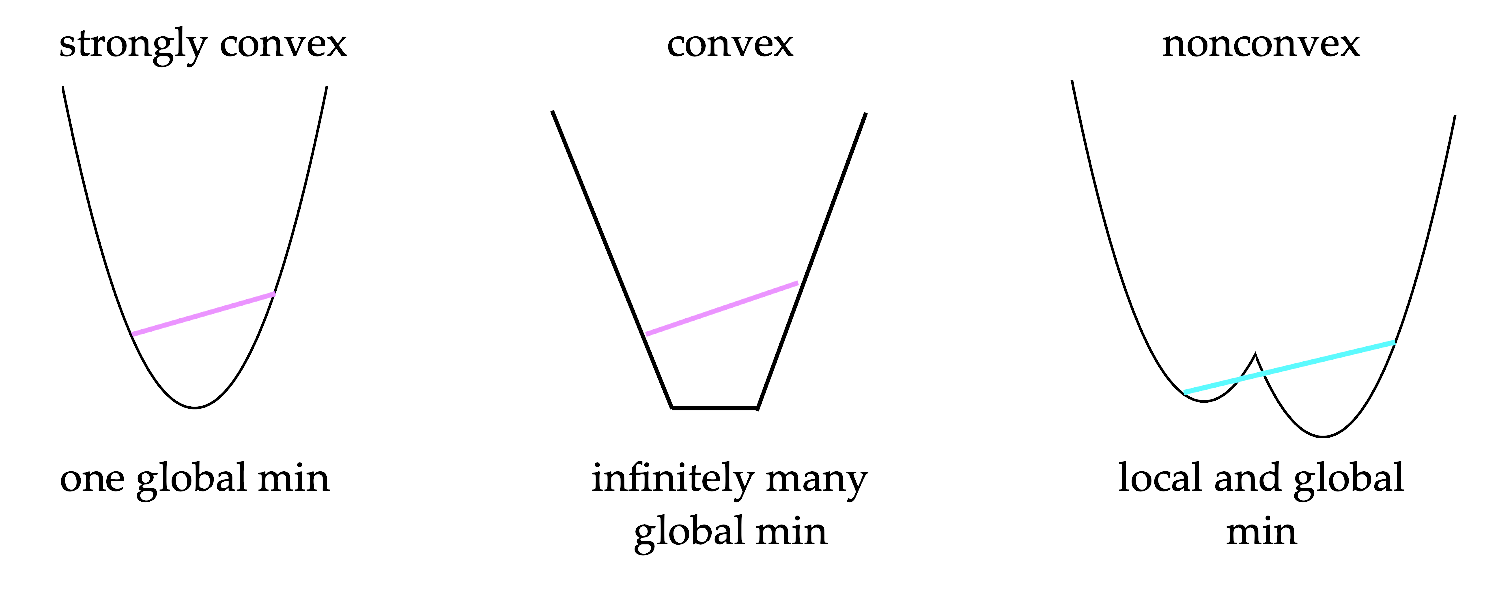
\includegraphics[width=3in]{graphics/convex.png}
\caption{Various functions and their (non) convexity properties.}
\end{figure}

LSR has a closed form solution $\hat{\theta}$ which is pretty rare; most complex models do not have a nice closed form solution. To find the closed form solution of $\hat{\theta}$, consider when the gradient of $\frac{1}{n}\sum_{i=1}^{n}(\theta^T x_i - y_i)$ w/rt to $\theta$ is 0.

\begin{align}
\nabla \frac{1}{n}\sum_{i=1}^{n}(\theta^T x_i - y_i) &= \frac{1}{n}\sum_{i=1}^{n} \nabla (\theta^T x_i - y_i)^2 \\
&= \frac{1}{n} \sum_{i=1}^{n} 2x_i(x_i^T \theta - y_i)
\end{align}

The gradient\footnote{We can move the transposes around since $\theta^Tx_i$ and $y_i$ are scalars.} is equal to 0 when 
$$\sum_{i=1}^{n} x_ix_i^T\hat{\theta} = \sum_{i=1}^n y_ix_i.$$

This is the \textit{first order optimality condition} for LSR. To solve for $\theta = \hat{\theta}$, let $X$ be a matrix where each row is a data point $x_i$ and $Y$ be a matrix where each row is a label $y_i$. Then, the first order optimality condition becomes

$$X^TX\hat{\theta} = X^T Y$$

If $X$ is full rank (i.e. the problem is not underspecified), then $X^TX$ is full rank and thus invertible. 
If $X$ is not full rank (i.e. the problem is underspecified), then we can use the psuedoinverse\footnote{Also called the Moore Penrose Inverse, see \url{https://en.wikipedia.org/wiki/Moore\%E2\%80\%93Penrose_inverse}. The pseudoinverse is denoted with $\dag$.} to get $\hat{\theta}$. Thus, 

$$\hat{\theta} = (X^TX)^{\dag}X^TY = (\sum_{i=1}^{n} x_i x_x^T)^{\dag} \sum_{i=1}^{n} y_ix_i.$$

The pseudoinverse has the nice property of producing the min-norm $\hat{\theta}$\footnote{Since the system is underspecified, there are infinitely many $\hat{\theta}$'s that achieve the minimum risk.}. This can be shown using Lagrange multipliers or projections among other methods. In the case of a fully specified system (i.e. $X^TX$ is invertible) then the pseudoinverse is the inverse and $\hat{\theta}$ is still the min-norm solution since there is only one solution.

Thus, we have derived the empirical risk minimizer for this least squares problem. 
Recall the fundamental theorem of machine learning.
What is the population risk?

Under a \textit{fixed design} generative model, the features describing the setup are fixed and like any other linear model:
\begin{theorem}
\begin{align*} 
y_{i} = \theta_{*}^{T}x_{i} + v_{i}
\end{align*}
\end{theorem}
$v_{i}$ is also i.i.d with a mean of $0$ and variance of $\sigma^{2}$. The excess risk is given by
\begin{theorem}
\begin{align*} 
R(\theta) = \frac{1}{n} \sum_{i=1}^{n}\mathop{{}\mathbb{E}}_{yi} [(x_{i})^{T}\theta - y_{i})^{2}]
\end{align*}
\end{theorem}
\begin{proof} We will prove that $R(\theta) = R(\hat{\theta)} - R(\theta_{*}) = \frac{\sigma^{2}d}{n}$ \\
Let's start with the theorem and work our way through. \\
\begin{align*}
\frac{1}{n}\sum_{i=1}^{N}\mathop{{}\mathbb{E}}_{yi}[(\theta^{T}x_{i} - (\theta_{*}^{T}x_{i}+v_{i}))^{2}] &= \frac{1}{n}\sum_{i=1}^{N}\mathop{{}\mathbb{E}}_{yi}[((\theta^{T} - \theta_{*}^{T})x_{i}+v_{i})^{2}] \\
&= \frac{1}{n}\sum_{i=1}^{N}\mathop{{}\mathbb{E}}_{yi}[((\theta^{T} - \theta_{*}^{T})x_{i})^{2}-2(\theta - \theta_{*})^{T}x_{i}v_{i}+v_{i}^{2}] \\
\end{align*}
The terms within the middle of the expectation are independent under a fixed setting and can be reduced to $0$, simplifying it further to \\
\begin{align*}
 \frac{1}{n}\sum_{i=1}^{N}\mathop{{}\mathbb{E}}_{yi}[(\theta^{T}x_{i} - (\theta_{*}^{T}x_{i}+v_{i}))^{2}] = \frac{1}{n}\sum_{i=1}^{N}\mathop{{}\mathbb{E}}_{yi}[((\theta^{T} - \theta_{*}^{T})x_{i})^{2}+\sigma^{2}] 
\end{align*}
Knowing that 
\begin{align*}
    \theta = (x^{T}x)^{-1}x^{T}y = (x^{T}x)^{-1}x^{T}(x\theta_{*}+v)
\end{align*}
The left side of the expectation can be reduced as follows:
\begin{align*}
\mathop{{}\mathbb{E}}||x(\theta-\theta_{*})||_{2}^{2} &=\mathop{{}\mathbb{E}}||x[(x^{T}x)^{-1}x^{T}(x\theta_{*}+v)-\theta_{*}]||_{2}^{2} \\
&=\mathop{{}\mathbb{E}}||x(x^{T}x)^{-1}x^{T}v||_{2}^{2}
\end{align*}
Substituting this back we can further proceed
\begin{align*}
\frac{1}{n}\mathop{{}\mathbb{E}}[v^{T}x(x^{T}x)^{-1}x^{T}x(x^{T}x)^{-1}x^{T}v] &= \frac{1}{n}\mathop{{}\mathbb{E}}[v^{T}x(x^{T}x)^{-1}x^{T}v] \\ 
&= \frac{1}{n}\mathop{{}\mathbb{E}}[v^{T}Pv] \\
&= \frac{1}{n}tr(p)\mathop{{}\mathbb{E}}[vv^{T}] \\ 
&= \frac{\sigma^{2}}{n}tr(p) \\
&= \frac{\sigma^{2}d}{n}
\end{align*}
\end{proof}
This intuitively makes sense as the more random the noise, the more the excess risk will be blown up. The more dimensions needed will also increase the excess risk displayed as it's more information to gather. Increasing the number of samples will also lower the excess risk to zero as you see a large number of more samples, your understanding of the true distribution will approach the optimal. 





\marginnote{Originally scribed by Eliot Shekhtman \& Yann Hicke on August 22nd, 2022 and Albert Tseng \& Kimia Kazemian on 8/24/2022}

\section{Exercises}
\begin{exercise}
for the same generative model and a new fixed $x_{n+1}$ what is the expected loss $\mathbb{E}_y[(\hat{\theta}^Tx_{n+1}-y_{n+1})^2]$? Can you interpret the quantities?
\end{exercise}
\begin{proof}
\begin{align*}
    \mathbb{E}_y[(\hat{\theta}^Tx_{n+1}-y_{n+1})]
    &=(\hat{\theta}^Tx_{n+1})^2-2\hat{\theta}^Tx_{n+1}\mathbb{E}_y[y_{n+1}]+\mathbb{E}[y_{n+1}^2] \\
    &=(\hat{\theta}^Tx_{n+1})^2-2\hat{\theta}^Tx_{n+1}\theta_{*}^Tx_{n+1}+(\theta_{*}^Tx_{n+1})^2 \\
    &=([\hat{\theta}^T-\theta_{*}^T]x_{n+1})^2\\
    &=([Y^TX(X^TX)^{\dag}-\theta_{*}^T]x_{n+1})^2\\
    &=([(\theta_{*}^TX^T+V^T)X(X^TX)^{\dag}-\theta_{*}^T]x_{n+1})^2\\
    &=(V^TX(X^TX)^{\dag}x_{n+1})^2
\end{align*}
so the expected loss is the squared error in our estimate at $x_{n+1}$, without considering the underlying noise.
\end{proof}

\subsection{Exercise}\label{sec:exercise}
For the same generative model and a new fixed $x_{n+1}$, what is the expected loss $\mathop{{}\mathbb{E}}_{y}[(\hat{\theta}^{T}x_{n+1} - y_{n+1})^{2}]$? Can we interpret these quantities.
\begin{align*} 
\mathop{{}\mathbb{E}}_{y}[(\hat{\theta}^{T}x_{n+1} - y_{n+1})^{2}] \\
= \mathop{{}\mathbb{E}}_{vi}[(\hat{\theta} - \theta_{*})^{T}x_{n+1} + v_{i})^{2}] \\ 
= \mathop{{}\mathbb{E}}_{vi}[(\hat{\theta} - \theta_{*})^{T}x_{n+1}] + (\mathop{{}\mathbb{E}}_{vi}[v_{i}^{2}]) \\ 
= ((\hat{\theta} - \theta_{*})^{2} + var(v_{i}) + (\mathop{{}\mathbb{E}}_{vi}[v_{i}])^{2} \\ 
= ((\hat{\theta} - \theta_{*})^{2} + \sigma^{2}
\end{align*}
These 2 terms can be interpreted as the bias squared (left term) and some irreducible error/noise (right term).
\smallbreak
In the \textit{random design} setting, we take each $x_{i}$ to be drawn i.i.d from $\mathcal{N}$($0$, $\Sigma$) and assume that $v_{i}$ is also Gaussian. The risk is then $R(\theta) = \mathbb{E}_{x,y}[(x^{T}\theta - y)^{2}]$. What is the excess risk of $\hat{\theta}$ in terms of $X^{T}X$ and $\Sigma$? What is the excess risk in terms of $\sigma^{2}, n, d$?
\begin{align*} 
\mathop{{}\mathbb{E}}[R(\hat{\theta}] - R^{*} &= \mathop{{}\mathbb{E}}||(X^{T}X)^{-1}X^{T}v||_{2}^{2} \\
&= \frac{1}{n}\mathop{{}\mathbb{E}}[v^{T}X(X^{T}X)^{-1}X^{T}X(X^{T}X)^{-1}X^{T}v] \\
&= \frac{1}{n}\mathop{{}\mathbb{E}}[v^{T}X(X^{T}X)^{-1}X^{T}v] \\ 
&= \frac{1}{n}\mathop{{}\mathbb{E}}[v^{T}Pv] \text{, where } P = X(X^{T}X)^{-1}X^{T} \\
&= \frac{1}{n}\mathop{{}\mathbb{E}}[tr(Pvv^{T})] \\
&= \frac{\sigma^{2}}{n}tr(P) \\
&= \frac{\sigma^{2}d}{n}
\end{align*}



